\section{Results and discussion}
\label{sec:eval:resultsdiscussion}

% ----------------------- paths to graphics ------------------------

\graphicspath{{6_evaluation/images/}}

% ----------------------- contents from here ------------------------
% 

TODO-1: short summary of the experiments and the results that will follow.

\subsection{VectorWise baseline results}
\label{subsec:eval:results:vectorwise}

We evaluated the \textit{whitebox compression} model against the \nameref{subsec:eval:methodology:vectorwise} according to the methodology (\ref{subsec:eval:methodology:vectorwise}). Figure~\ref{fig:eval:results:vectorwise:total} shows the compression ratios---\(ratio_{blackbox}\), \(ratio_{whitebox}\)---and the 3 sizes they were derived from---\(size_{uncompressed}\), \(size_{blackbox}\), \(size_{whitebox}\)---for each table. The tables are sorted in descending order by \(ratio_{whitebox}\). In this figure we made the comparison for the full tables, including all logical columns, even though only a part of them are in the scope of \textit{whitebox compression}.

\begin{figure}[h]
  \centering
   \makebox[\textwidth][c]{
    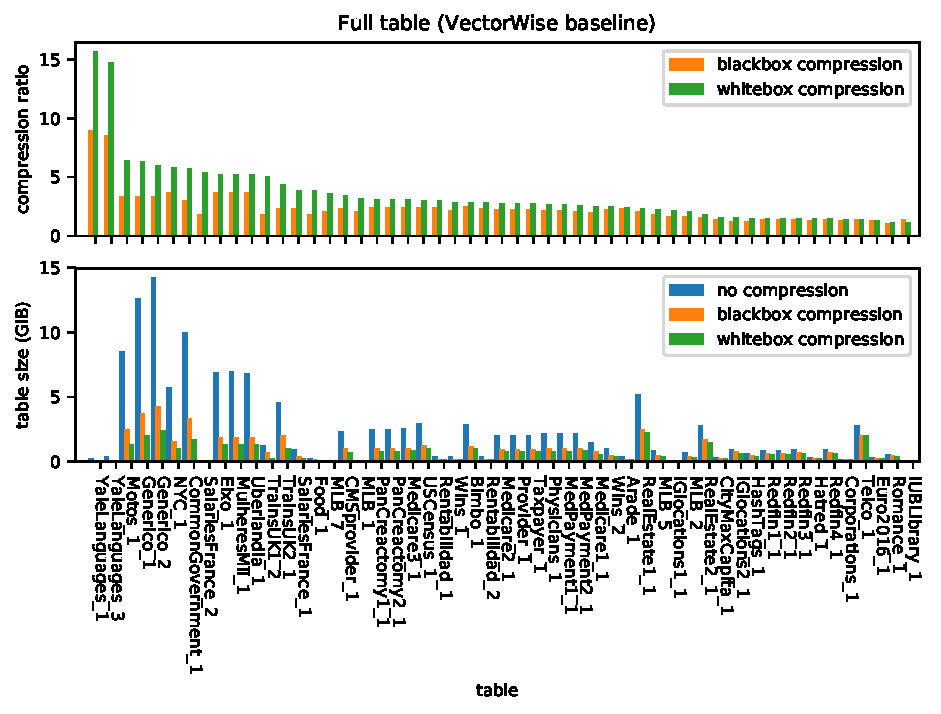
\includegraphics[width={1.1\linewidth}]{6_evaluation/images/vw_total.pdf}
    }
  \caption{Full table comparison (VectorWise baseline)}
  \label{fig:eval:results:vectorwise:total}
\end{figure}

The total size of the uncompressed tables is 131GB. The overall compression ratios are:  \(ratio_{blackbox} = 2.58\) and \(ratio_{whitebox} = 3.58\). \textit{Whitebox compression} has an overall ratio of 1.38 against blackbox compression. In the first chart we can observe that for one third of the tables \(ratio_{whitebox}\) is significantly higher than \(ratio_{blackbox}\). The rest of the tables have similar compression ratios. 
An important observation is that, even though \textit{whitebox compression} only brings a significant improvement to a small part of the tables, it is never worse than blackbox compression. The only exception is the last table, where \(ratio_{blackbox} = 1.38\) and \(ratio_{whitebox} = 1.11\). However, this table is extremely small in uncompressed format: 508KB. Such small data already fits in the CPU cache and does not require compression at all. We can further notice that most of the tables with high \(ratio_{blackbox}\) have even higher \(ratio_{whitebox}\) and those with the lowest \(ratio_{blackbox}\) have the lowest \(ratio_{whitebox}\). A possible explanation for this phenomenon is that \textit{whitebox compression} exploits the same columns as blackbox compression and improves the compression ratio. From the second chart we can make the observation that the majority of the large tables tend to have higher compression ratios than most of the small tables, with some exceptions. This is particularly true for \textit{whitebox compression}, but also for blackbox, since the two are also somewhat correlated.

These results include all the logical columns, even tough some of them were not represented through \textit{whitebox compression}. Our compression model does not incur any overhead on these columns and therefore we can exclude them from the evaluation with the purpose of measuring the improvement more accurately. Figure~\ref{fig:eval:results:vectorwise:used} shows the same charts but only includes the columns represented through \textit{whitebox compression}. This analysis required column -level analysis. For this reason we excluded the tables for which we couldn't match the columns with VectorWise's data files---because of multiple columns stored in the same file. Tables are sorted by the new \(ratio_{whitebox}\).

\begin{figure}[h]
  \centering
   \makebox[\textwidth][c]{
    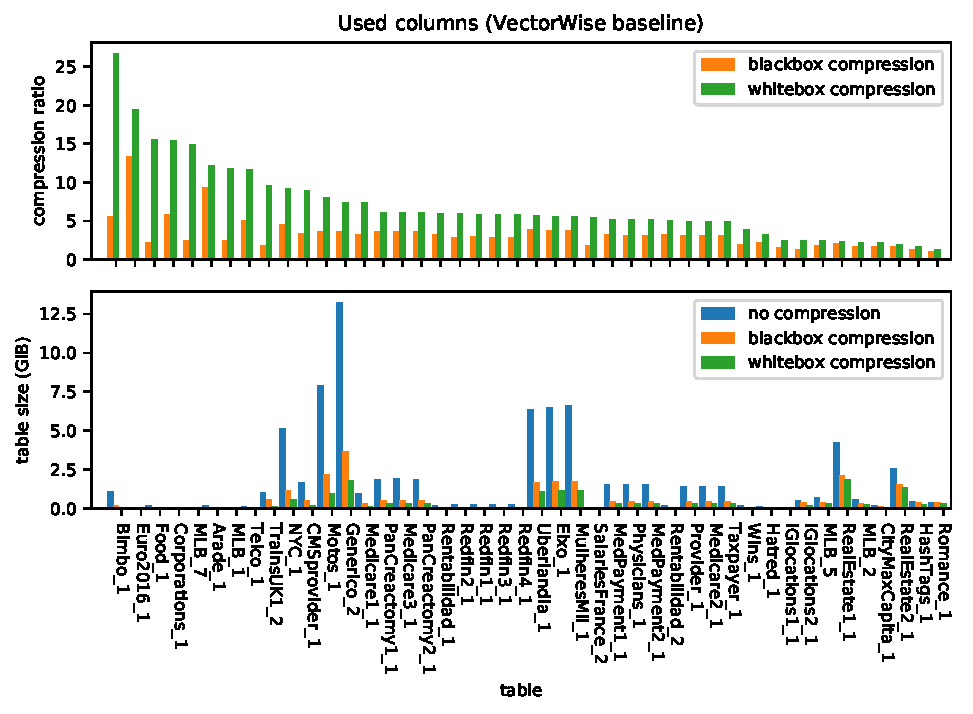
\includegraphics[width={1.1\linewidth}]{6_evaluation/images/vw_used.pdf}
    }
  \caption{Used columns comparison (VectorWise baseline)}
  \label{fig:eval:results:vectorwise:used}
\end{figure}

The results are as expected: the average compression ratio increased and \textit{whitebox compression} brings a significant improvement for the majority of the tables. Table~\ref{tab:eval:results:vectorwise:totalvsused} shows an overall comparison between the full table results and the used columns results.

\begin{table}[!h]
\centering
\begin{tabular}{c|cccc}
             & \begin{tabular}[c]{@{}c@{}}\(size_{uncompressed}\)\\ (GB)\end{tabular} & \(ratio_{blackbox}\) & \(ratio_{whitebox}\) & \(\frac{ratio_{blackbox}}{ratio_{whitebox}}\) \\ \hline
Full table   & 131                                                                    & 2.58                 & 3.58                 & 1.38                                          \\
Used columns & 77                                                                     & 3.16                 & 5.16                 & 1.63                                         
\end{tabular}
\caption{Full table vs. used columns (VectorWise baseline)}
\label{tab:eval:results:vectorwise:totalvsused}
\end{table}

Only 68\% of the total size of the data was represented through \textit{whitebox compression}. The increase of \(ratio_{blackbox}\) shows that columns used by \textit{whitebox compression} are also good candidates for  blackbox compression. However, \(ratio_{whitebox}\) increased more than \(ratio_{blackbox}\), indicating that \textit{whitebox compression} created opportunities for more compact representation.

The difference between the used columns evaluation and the full table evaluation is determined by the lack of opportunities for \textit{whitebox compression} in part of the data. For a better understanding, imagine that we want to compress 2 columns \(c_{a}\) and \(c_{b}\) of equal size \(s\). \(c_{a}\) presents no compression opportunities (\(ratio_{a} = 1\)) and \(c_{b}\) has \(ratio_{b} = 10\). Even though half of the data is highly compressible, the total ratio of the 2 columns is much lower: \(ratio_{total} = \frac{2 \times s}{s + 0.1 \times s} = 1.81\).

The conclusion that we can draw so far is that \textit{whitebox compression} achieves high compression ratios on the columns that it represents through the expression trees and is never worse than blackbox compression alone. Additionally, the columns that do not present compression opportunities are not affected and the underlying database system operates normally on them.


% ------------ estimator model ------------ %

\subsection{Estimator model baseline results}
\label{subsec:eval:results:estimator}

We conducted an additional evaluation of the \textit{whitebox compression} model, this time against the \nameref{subsec:eval:methodology:estimator}, with the purpose of measuring the compression capabilities of a stand-alone \textit{whitebox} system. The VectorWise blackbox compression schemes are replaced by the lightweight compression estimators defined in \ref{sub:estimators}. We followed the methodology described in \ref{subsec:eval:methodology:estimator}. Figure~\ref{fig:eval:results:estimator:used} shows the compression ratios and table sizes, considering only the columns represented through \textit{whitebox compression}.

\begin{figure}[h]
  \centering
   \makebox[\textwidth][c]{
    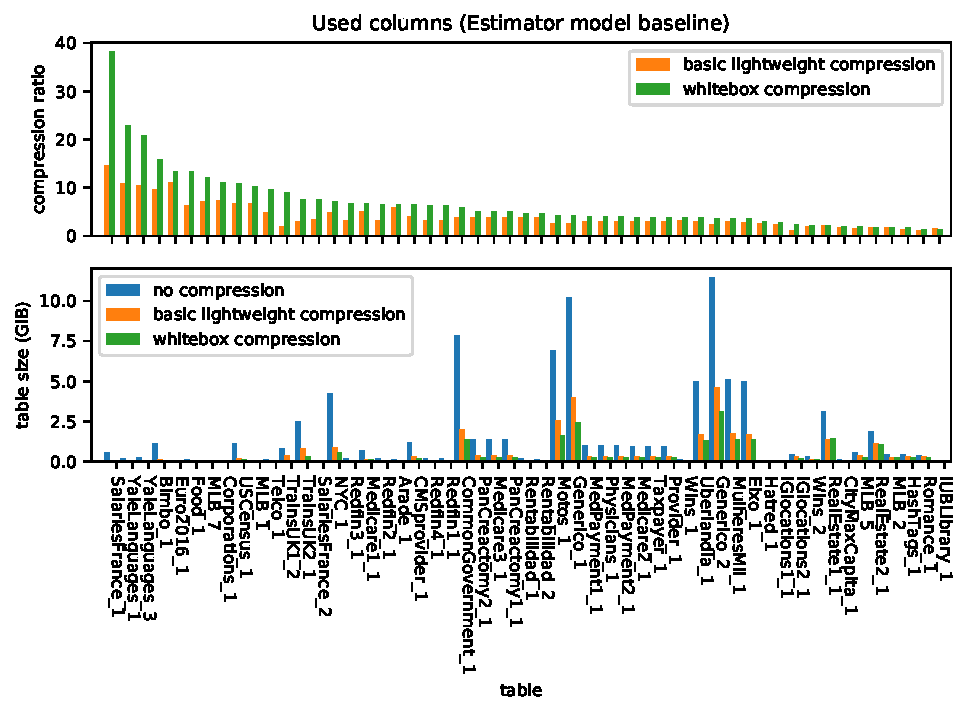
\includegraphics[width={1.1\linewidth}]{6_evaluation/images/estimator_used.pdf}
    }
  \caption{Used columns comparison (Estimator model baseline)}
  \label{fig:eval:results:estimator:used}
\end{figure}

The overall results are similar to the \nameref{subsec:eval:methodology:vectorwise}: \textit{whitebox compression} is effective for part of the tables (around 40\% of them in this case) and for the rest of them it gives similar compression ratios with the basic lightweight schemes. Similarly, the compression ratios are correlated---\(ratio_{whitebox}\) is higher respectively lower where \(ratio_{lightweight}\) is higher respectively lower. The same observation---that \textit{whitebox compression} is never worse than the basic lightweight compression schemes alone---is also true for the estimator baseline---with the same exception: the last table. Table~\ref{tab:eval:results:estimatorvsvectorwise} shows an overall comparison between the 2 baselines.

\begin{table}[!h]
\centering
\begin{tabular}{c|cccc}
                & \begin{tabular}[c]{@{}c@{}}\(size_{uncompressed}\)\\ (GB)\end{tabular} & \(ratio_{blackbox}\) & \(ratio_{whitebox}\) & \(\frac{ratio_{blackbox}}{ratio_{whitebox}}\) \\ \hline
VectorWise      & 77                                                                     & 3.16                 & 5.16                 & 1.63                                          \\
Estimator model & 83                                                                     & 2.87                 & 4.04                 & 1.40                                         
\end{tabular}
\caption{VectorWise baseline vs. estimator model baseline (used columns)}
\label{tab:eval:results:estimatorvsvectorwise}
\end{table}

The total size of the used columns is 7\% higher and the compression ratios decreased with 9\% for the lightweight schemes and 21\% for \textit{whitebox compression}. The improvement of \textit{whitebox compression} is also a bit lower (14\% decrease). The \nameref{subsec:eval:methodology:estimator} seems to reduce the impact of both compression systems and in particular the effect of our model. However, the objective of \textit{whitebox compression}---to create compression opportunities for more compact data representation---is still met, since it brings an increase in compression ratio from 2.87 to 4.04.

Figure~\ref{fig:eval:results:estimatorvsvw} creates a better picture of the differences between the 2 baselines---a comparison of the table sizes for the three metrics in the methodology: \(size_{uncompressed}\), \(size_{lightweight}\)/\(size_{blackbox}\) and \(size_{whitebox}\).

\begin{figure}[h]
  \centering
   \makebox[\textwidth][c]{
    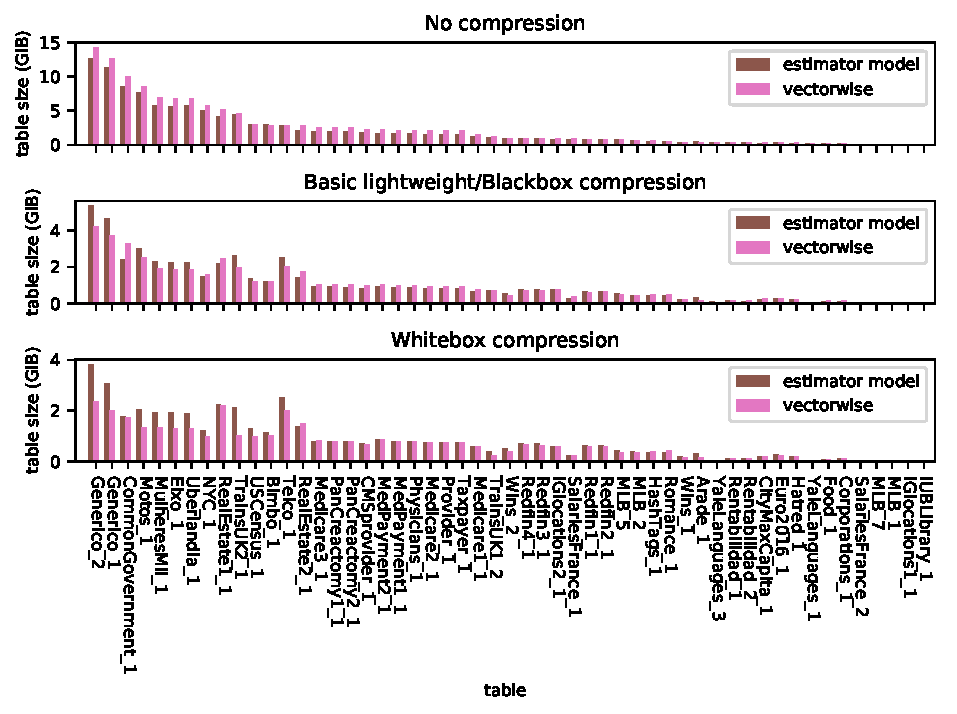
\includegraphics[width={1.1\linewidth}]{6_evaluation/images/estimator_vs_vw_combined.pdf}
    }
  \caption{Baseline comparison (full table): Estimator model vs. Vectorwise}
  \label{fig:eval:results:estimatorvsvw}
\end{figure}

In the first chart we can see that the estimated uncompressed size of the data is a bit smaller than the VectorWise size for most tables. This result is not unexpected, since the storage layer of a real system is more complex and might add additional overhead compared to the theoretical estimation that we made. Moreover, the exact representation of each data type might differ from the one that we used. The second chart shows how VectorWise's blackbox compression schemes perform better than the (estimated) lightweight compression methods for some tables. This is not a surprising result, since our lightweight compression schemes are not optimized and the exception handling mechanism is different. A somewhat unexpected result can be observed in the third chart: VectorWise is even better at compressing the whitebox representation of the data than the estimator model for some tables. A possible explanation might be that the number, type and size of columns differ, as \textit{whitebox compression} creates many nullable columns because of the exception handling mechanism. Moreover, the compression metadata differs and its size is estimated in a different way. An additional notable observation is that the difference between VectorWise and the estimator model is usually higher where the size of the data is larger, while for smaller tables the 2 models give closer results.

The overall conclusion that we can draw from this experiment is that, even though the 2 models give somewhat different results, \textit{whitebox compression} still brings a significant improvement over the existing lightweight compression methods. The main reason for the lower compression ratios of the \nameref{subsec:eval:methodology:estimator} is the different---and unoptimized---compression schemes. A more thorough experiment and analysis needs to be performed in order to properly evaluate the performance of a stand-alone \textit{whitebox} system in practice---we leave this for future work. Even so, we showed that \textit{whitebox compression} can be used to enhance existing systems---like VectorWise---as an intermediate layer before the optimized compression methods.


% ------------ analysis ------------ %

\subsection{Results analysis}
\label{subsec:eval:results:analysis}

To better understand the impact of \textit{whitebox compression} and how it represents the data, we performed an analysis of the physical data size components and the expression trees. We conducted this analysis on the results obtained with the VectorWise methodology (\ref{subsec:eval:methodology:vectorwise}).

Figure~\ref{fig:eval:results:useddatatypes} presents the distribution of datatypes across the logical columns represented through \textit{whitebox compression}. The majority of columns are \verb|VARCHAR|, since our system leverages the opportunities present in strings. The rest of the columns are numeric and boolean and are all constant columns, since the \nameref{subsec:pd:constant} pattern detector is the only one that works on other datatypes than strings. Figure~\ref{fig:eval:results:outdatatypes} shows the distribution of datatypes across the physical columns resulted after the \textit{whitebox} representation (excluding columns). With the exception of 1\% \verb|VARCHAR| columns, all the other are numeric. They resulted from \nameref{subsec:pd:numericstrings} and \nameref{subsec:pd:dict} representations (observation: dictionary ids are stored in SQL numeric datatypes so that they can be loaded into VectorWise; however, the main purpose of \nameref{subsec:pd:dict} expression nodes is to serve as an intermediates representation layer before \nameref{subsec:pd:columncorrelation}). The only pattern detector that outputs \verb|VARCHAR| columns is \nameref{subsec:pd:charsetsplit}. The other 2 pattern detectors---\nameref{subsec:pd:constant} and \nameref{subsec:pd:columncorrelation}---do not output any physical columns. Instead, they reduce the number of columns by consuming them and only storing metadata.

\begin{figure}[h]
  \centering
  \makebox[\textwidth][c]{
  \begin{subfigure}[t]{0.6\linewidth}
    \centering
    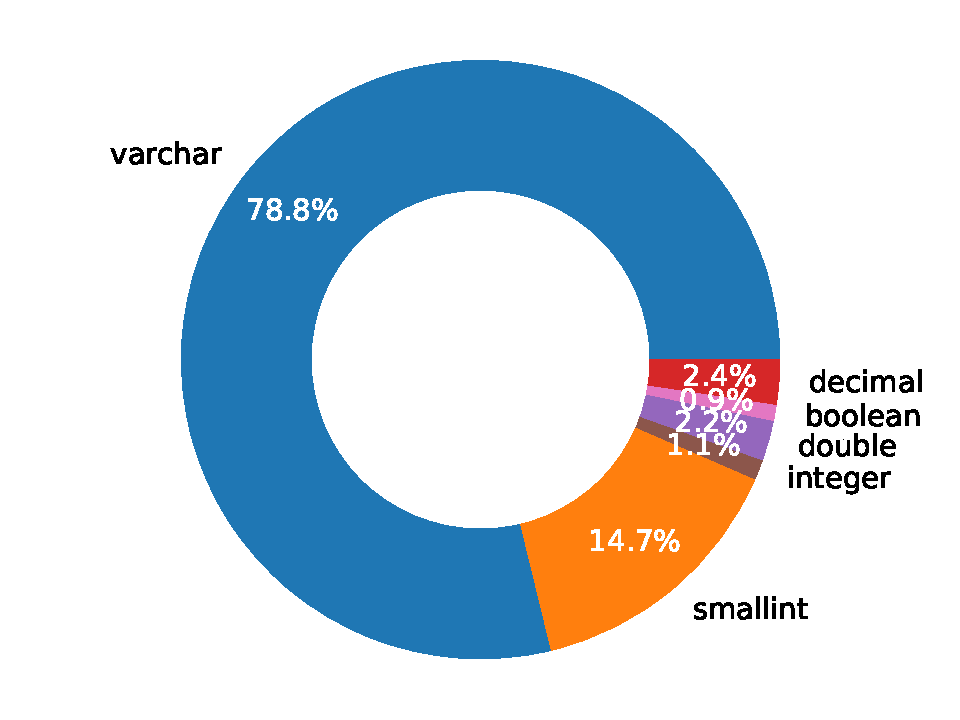
\includegraphics[width=1\linewidth]{6_evaluation/images/used_datatypes.pdf}
    \caption[b]{Logical columns (used)}
    \label{fig:eval:results:useddatatypes}
  \end{subfigure}
%   \hspace{1em}
  \begin{subfigure}[t]{0.6\linewidth}
    \centering
    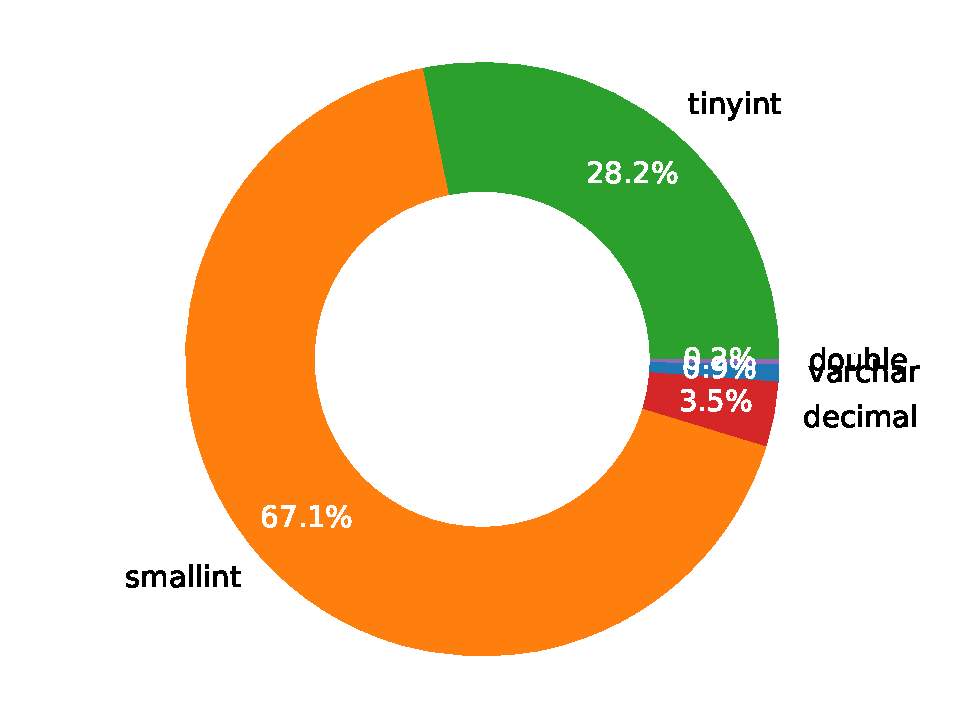
\includegraphics[width=1\linewidth]{6_evaluation/images/out_datatypes.pdf}
    \caption[b]{Physical columns}
    \label{fig:eval:results:outdatatypes}
  \end{subfigure}
  }
  \caption{Column datatype distribution}
  \label{fig:eval:results:columndatatypes}
\end{figure}

Table~\ref{tab:eval:results:analysis2} shows the impact of \textit{whitebox compression} through an analysis of the logical and physical columns in terms of numbers and sizes. 

\begin{table}[!h]
\centering
\begin{tabular}{cc|c|cc}
                         &           & Logical columns & \multicolumn{2}{c}{Physical columns} \\
                         &           & Used columns    & Data columns   & Exception columns   \\ \hline
\multirow{2}{*}{Average} & Count     & 26              & 8              & 46                  \\
                         & Size (MB) & 1.45GB          & 85MB           & 262MB               \\ \hline
\multirow{2}{*}{Total}   & Count     & 1406            & 462            & 2479                \\
                         & Size      & 77.2GB          & 3.7GB          & 11.3GB             
\end{tabular}
\caption{Logical vs. physical columns}
\label{tab:eval:results:analysis1}
\end{table}

On the average table, there are 26---out of 67 (38\%)---logical columns used in the \textit{whitebox} representation. They are represented through only 8 physical columns containing compressed data and an additional 46 exception columns. The number of data columns is reduced because of the expression nodes that consume columns: \nameref{subsec:pd:constant} and \nameref{subsec:pd:columncorrelation}. The number of exception columns is very high due to our option to keep an exception column for each expression node in the tree and to allow recursive compression of exception columns. However, these columns are very sparse and contain mostly null values---which are effectively stored by the underlying database system through a bitmap. In terms of size, the average of 1.45GB of input data is represented through only 85MB of compressed data and 262MB of exceptions. Therefore, 1.19GB of the data (non-exceptions: 1.45GB - 262MB) is represented through 85MB of compressed data---plus the size of the metadata, which is insignificant (see Figure~\ref{fig:eval:results:outsizedistribution}). These results show the high degree of redundancy present in real data---and that we can squeeze this redundancy out of the data if we have a proper exception handling mechanism.
Table~\ref{tab:eval:results:analysis2} also shows the same analysis for the overall results---total of all tables---instead of the average.

Figure~\ref{fig:eval:results:outsizedistribution} shows a better picture of the physical data size distribution and the components that make it up. The exceptions sum up to 75.3\% while the compressed data represents 24.5\% of the total physical data size. The compression metadata (e.g. dictionaries, correlation maps, etc.) is insignificant, since we used a single compression tree for the entire table. The alternative---handling blocks of data separately---would allow a more fined grained representation with possibly simpler compression trees, at the expense of increasing the total metadata size.

\begin{figure}[h]
\centering
\makebox[\textwidth][c]{
\begin{minipage}{0.55\textwidth}
  \centering
  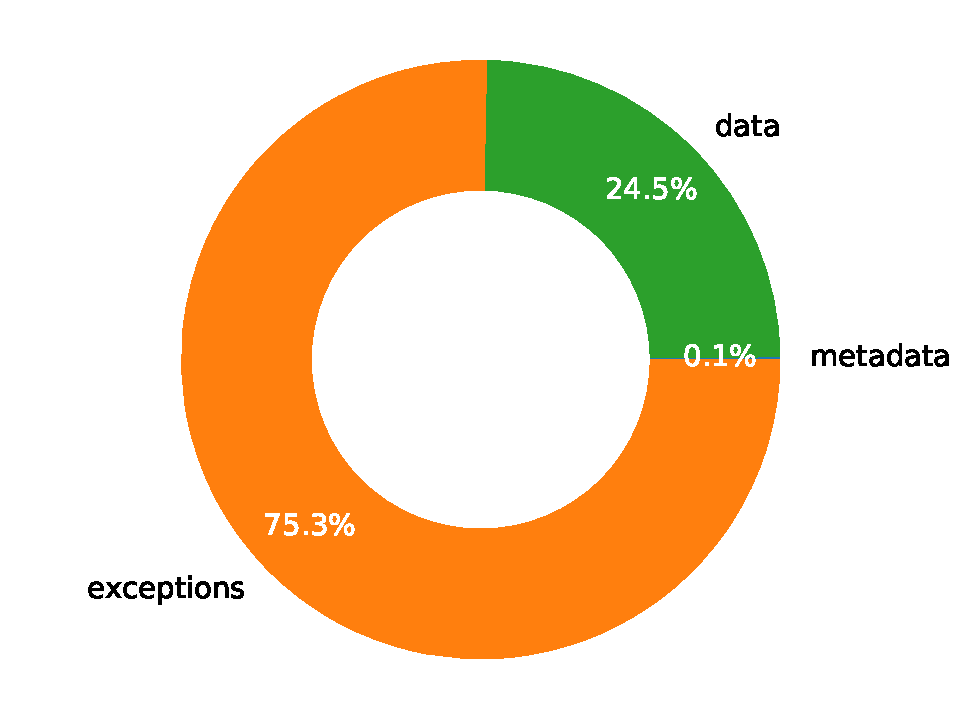
\includegraphics[width={1.0\linewidth}]{6_evaluation/images/out_size_distribution.pdf}
  \caption{Physical size distribution}
  \label{fig:eval:results:outsizedistribution}
\end{minipage}
% \hspace{1em}
\begin{minipage}{0.55\textwidth}
  \centering
  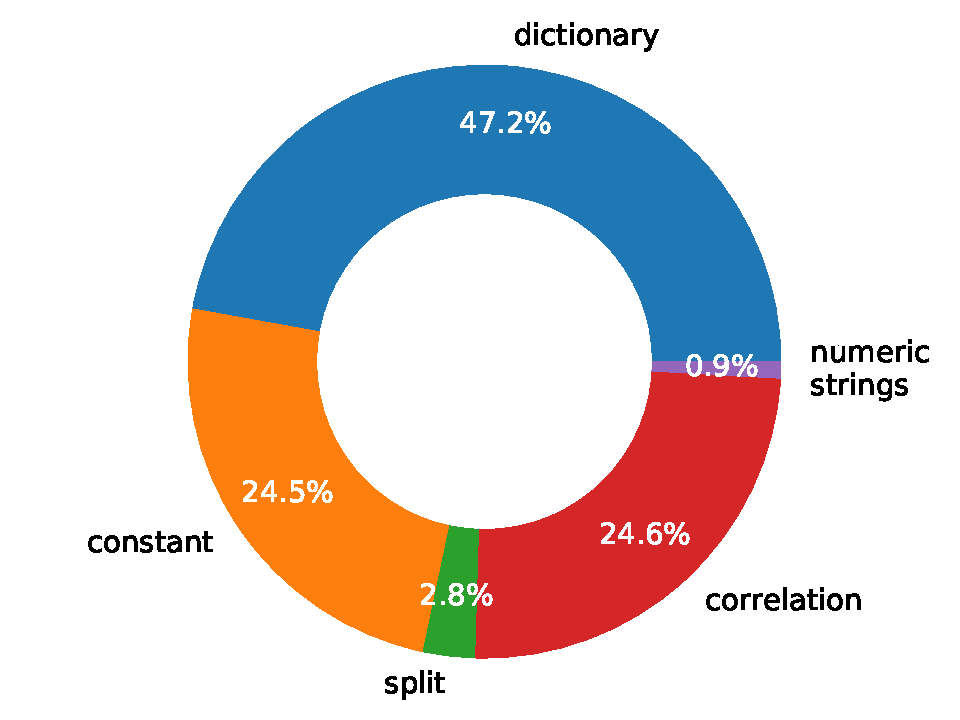
\includegraphics[width={1.0\linewidth}]{6_evaluation/images/expr_n_types.pdf}
  \caption{Expression node types distribution}
  \label{fig:eval:results:exprntypedistribution}
\end{minipage}
}
\end{figure}

For the rest of our analysis we focused our attention to the expression trees. Recall that the so called expression tree is actually and acyclic directed graph with root nodes and multiple connected components (\ref{ch:exprlang}~\nameref{ch:exprlang}). Each connected component represents a subset of the logical columns as a function of physical columns. Table~\ref{tab:eval:results:analysis2} shows the characteristics of the average expression tree.

\begin{table}[!h]
\centering
\begin{tabular}{c|cccc}
Connected components   & Expression nodes & Depth & Logical columns & Physical columns \\
(on average per table) & \multicolumn{4}{c}{(on average per connected component)}  \\ \hline
12.5                   & 3.3              & 1.4   & 1.7           & 0.8           
\end{tabular}
\caption{Expression tree statistics}
\label{tab:eval:results:analysis2}
\end{table}


There are 12.5 connected components, with an average of 3.3 expression nodes and a depth of 1.4 levels. This shows that expression trees are not very complex and relatively fast to evaluate. A connected component represents on average 1.7 logical columns as a function of 0.8 physical columns (excluding exception columns)---the 0.8 value is due to the expression nodes that do not output any physical columns: \nameref{subsec:pd:constant} and \nameref{subsec:pd:columncorrelation}. Here we see again the capacity of \textit{whitebox compression} to reduce the number of columns by storing metadata instead.
% Moreover, the dependencies between columns are not that high, given the small number of logical and physical columns.
% However, these results are showing the average. There are many complex connected components and even more simple ones with only one expression node.

TODO-1: create histograms with the values in Table~\ref{tab:eval:results:analysis2}.

Finally, Figure~\ref{fig:eval:results:exprntypedistribution} shows the distribution of the expression node types in the average expression tree. In this analysis we considered both internal and leaf nodes. We notice that the majority is composed of \nameref{subsec:pd:constant}, \nameref{subsec:pd:dict} and \nameref{subsec:pd:columncorrelation}, while only a small percentage are \nameref{subsec:pd:charsetsplit} and \nameref{subsec:pd:numericstrings}. This is due to the high \nameref{subsec:pd:dict} compression potential of the data and to the high correlation---high redundancy in other words. An additional reason is the priority configuration that we used for this experiment---recall that \nameref{subsec:pd:constant} and \nameref{subsec:pd:dict} have the highest priority (\ref{sec:eval:expsetup}~\nameref{sec:eval:expsetup}). Also note that all \nameref{subsec:pd:columncorrelation} nodes take as input---and consume---\nameref{subsec:pd:dict} expression nodes. Therefore, the majority of the \nameref{subsec:pd:dict} nodes are internal nodes of the expression tree. We also experimented with other learning configurations which resulted in more even distributions of the expression node types, but decided to show the results of this configuration because they were better. From our experiments we concluded that data can be represented and compressed in many ways. However, the learning algorithm needs to choose a single data representation, ideally the one that gives the smallest physical size.

The take-away message from this analysis is that we can represent many logical columns---mostly \verb|VARCHAR|---as functions of fewer physical columns---mostly numeric---at the expense of many exception columns---mostly nulls---and achieve high compression ratios---all of this automatically learned.

% TODO-2: new subsection about decompression implementation to validate input data reconstruction

% ---------------------------------------------------------------------------
% ----------------------- end of thesis sub-document ------------------------
% ---------------------------------------------------------------------------